\chapter{The model}
\label{chap:growing}

We model the economy as a network of interacting firms whose sizes evolve by Generalized
Lotka--Volterra dynamics. The standard form of these dynamics cannot represent a growing
economy, and this chapter builds the model that can by changing the standard form one step at a
time, fixing each defect as it appears. The result is then analysed in
Section~\ref{sec:model-phases}, where we locate the growing, fluctuating regime in which the
firm-growth statistics of Chapter~\ref{chap:firmgrowth} are measured.

\section{From Lotka--Volterra to the relative model}
\label{sec:relative-model}

We take as our starting point the Generalized Lotka--Volterra (GLV) system. Each firm $i$
carries a size $x_i \ge 0$ that grows logistically and is coupled to the others through a signed
interaction matrix,
\begin{equation}
    \dot{x}_i = x_i \left( 1 - x_i + (Wx)_i \right),
    \label{eq:abs-glv}
\end{equation}
with $W_{ij} = A_{ij}\,\alpha_{ij}$ on a sparse configuration-model graph. Here $A_{ij}$ is the
adjacency matrix of the graph, $1$ where firms $i$ and $j$ are connected and $0$ otherwise, and
$C$ is the mean degree. The coupling strengths are
$\alpha_{ij} = \mu/C + (\sigma/\sqrt{C})\,z_{ij}$, where the $z_{ij}$ are independent standard
Gaussian variables, drawn once for each graph and then held fixed, the quenched disorder of the
model. So $\mu$ sets the mean interaction, cooperative for $\mu > 0$ and competitive for
$\mu < 0$, and $\sigma$ its disorder.

Equation~\eqref{eq:abs-glv} cannot serve as it stands, and it fails for two reasons. First, it carries an absolute scale of size that an
economy does not have. The self-limitation $-x_i$ caps an isolated firm at $x_i = 1$, and the
quadratic interaction fixes once and for all the size at which growth, competition and
self-limitation balance. A real economy has no such reference size. Its output has grown by
orders of magnitude over two centuries while the distribution of firm sizes and the statistics
of their growth stayed essentially stationary, so the dynamics should be invariant under a
rescaling $x \to c\,x$ of the whole economy, which \eqref{eq:abs-glv} is not. Held at its
cooperative critical point the absolute model does grow without bound, but through a finite-time
blow-up of the total abundance rather than steady growth. Second, even at that point it delivers
only one of the two firm-growth facts. It reproduces the fat-tailed growth-rate distribution on
heterogeneous graphs, but its size--variance relation is not a stationary law, only a transient
traced out as an arbitrary initial condition relaxes onto the critical attractor, after which
every growth rate vanishes. We need, then, two things the absolute model lacks, invariance under
rescaling and a state that keeps fluctuating rather than relaxing.

Both follow from a single change. We let the self-limitation and the interactions act on the
size of a firm relative to the average firm $m = M/N = \langle x\rangle$ rather than on its
absolute size. Keeping the same interaction matrix $W$, the model becomes
\begin{equation}
    \dot{x}_i = x_i \left( 1 - \frac{x_i}{m} + \frac{(Wx)_i}{m} \right),
    \qquad m = \frac{1}{N}\sum_j x_j .
    \label{eq:relative-glv}
\end{equation}
The only change from \eqref{eq:abs-glv} is the two factors of $1/m$, but it makes the right-hand
side homogeneous of degree one in $x$. Under $x \to c\,x$ the mean $m$ scales in the same way,
the ratios $x_i/m$ and $(Wx)_i/m$ are unchanged, and the whole equation simply rescales, so that
if $x(t)$ is a solution then so is $c\,x(t)$. The economy no longer has a preferred size. The
change is also the economically natural one. A competitor's pressure on firm $i$ is now set by
its market share $x_j/m$ rather than by its absolute size, and a firm's own crowding is measured
against the typical firm rather than against a fixed ceiling, so what drives the dynamics is
relative standing in the market. The intrinsic Malthusian rate $1$ is left untouched and remains
the engine of growth, while the interactions, now made relative, only regulate it.

Two consequences of this change set up the rest of the model. The first is steady growth. Writing
$x_i = M y_i$ with $y$ on the simplex and the shorthands
$y^{\!\top} W y = \sum_{i,j} y_i W_{ij} y_j$, $y^{\!\top} y = \sum_i y_i^2$, the sum of
\eqref{eq:relative-glv} over $i$ gives
\begin{equation}
    \dot{M} = M \left[\, 1 + N\big( y^{\!\top} W y - y^{\!\top} y \big)\,\right]
            \equiv M\, g_{\mathrm{eff}}(y).
    \label{eq:Mdot-relative}
\end{equation}
Summing the absolute model \eqref{eq:abs-glv} instead leaves a right-hand side with a term in
$M^2$, the quadratic feedback responsible for the finite-time singularity. Dividing the
interactions by $m$ removes one power of $M$, the quadratic term becomes linear, and
\eqref{eq:Mdot-relative} is the equation of plain exponential growth,
$M(t) \sim e^{g_{\mathrm{eff}} t}$, with no singularity. In the regime we work in
$g_{\mathrm{eff}}$ settles to a small positive constant, so the economy grows at a steady rate
over unbounded physical time.

The second consequence concerns the shape. From \eqref{eq:relative-glv} and the quotient rule
the shares obey $\dot{y}_i = y_i ( f_i - \langle f \rangle )$ with the linear fitness
$f_i = 1 - N y_i + N (Wy)_i$ and $\langle f \rangle = \sum_j y_j f_j = g_{\mathrm{eff}}$. This is
a replicator equation, the canonical description of frequency-dependent selection, in which a
firm gains share precisely when its fitness exceeds the market average $\langle f \rangle$, and
it is the standard correspondence between Lotka--Volterra and replicator dynamics
\citep{hofbauer81}. Because the relative model does not blow up, it is written in the same
physical time $t$ in which $M$ grows, with no time rescaling. Above the disorder threshold
$\sigma_c = \sqrt{2}$ \citep{diederich1989} the replicator flow does not relax to a fixed point
but stays chaotic, so the growth rates $\dot y_i / y_i = f_i - \langle f\rangle$ never vanish.
This is the persistently fluctuating state we needed.

The chaotic flow has one feature that has to be controlled. Left to itself it drives some shares
arbitrarily close to zero, and a share that reaches zero stays there, so diversity erodes and the
state never becomes stationary. As is standard in the disordered Lotka--Volterra literature
\citep{bunin2017,roy2020} we add a small immigration term that pulls each share gently toward
$1/N$, setting a floor of rarity below which a firm cannot fall and preventing exact extinction.
The shape dynamics we integrate are then
\begin{equation}
    \begin{gathered}
        \dot{y}_i = y_i \left( f_i - \langle f \rangle \right) + \lambda\!\left( \tfrac{1}{N} - y_i \right), \\
        f_i = 1 - N y_i + N (Wy)_i,
        \qquad \langle f \rangle = \sum_j y_j f_j = g_{\mathrm{eff}},
    \end{gathered}
    \label{eq:replicator}
\end{equation}
with a rate $\lambda = 10^{-3}$. The immigration term conserves $\sum_i y_i = 1$, so it leaves
the growth equation \eqref{eq:Mdot-relative} untouched; in size-space it is the scale-invariant
influx $\dot{x}_i = x_i ( 1 - x_i/m + (Wx)_i/m ) + \lambda(m - x_i)$, an entry of small firms at a
rate set by the size of the economy itself.

One element of the model is still unspecified, the disorder normalization, and it is what
controls the firm-growth statistics of the next chapter, so we set it out now. On a heterogeneous
graph the natural per-firm choice normalizes each firm's couplings by its own degree $k_i$,
\begin{equation}
    \alpha_{ij} = \frac{\mu}{k_i} + \frac{\sigma}{\sqrt{k_i}}\,z_{ij},
    \label{eq:normalizations}
\end{equation}
with $k_i$ the degree of firm $i$ and the $z_{ij}$ the same standard Gaussian disorder as above.
This is the per-fan-in scaling,
in which both the mean pressure and the disorder are shared over a firm's own neighbours, so that
every firm carries a field of the same variance whatever its connectivity. On a regular graph it
reduces to the global normalization by the common degree, which is the case the mean-field theory
of Appendix~\ref{app:dmft} solves; the two differ on the heterogeneous graphs we use for the
measurements, where the own-degree choice is the one that keeps the disorder field comparable
across firms of unequal connectivity.

We integrate \eqref{eq:replicator} together with $\mathrm{d}\ln M/\mathrm{d}t = g_{\mathrm{eff}}$
directly in physical time, keeping the shape on the bounded simplex and the scale in its
logarithm so that nothing overflows however large $M$ becomes; the explicit solver and its cost
are specified in Appendix~\ref{app:numerics}.

\section{Phases of the model}
\label{sec:model-phases}

Before measuring the firm-growth statistics it helps to see where in parameter space the
growing, fluctuating state lives. Figure~\ref{fig:phase-diagram} maps the behaviour of the model
over the plane of the mean interaction $\mu$ and the disorder $\sigma$, classified from the
late-time dynamics of many graph realizations. Two genuine transitions organize it. The
dynamical threshold $\sigma_c = \sqrt{2}$ separates a frozen regime below, where the shape
relaxes to a fixed point and the growth rates vanish, from the chaotic regime above, where it
never settles. Cutting across it, the line $g_{\mathrm{eff}} = 0$ separates a growing economy
from a shrinking one. Where the competition is strong and the disorder high, coexistence
collapses and the dynamics either condense onto a few firms or grow explosively. The firm-growth
statistics of this thesis belong to the chaotic, growing band, the wedge bounded below by
$\sigma_c$, on one side by the $g_{\mathrm{eff}} = 0$ line, and on the other by the condensed
corner. This is an extended region rather than an isolated point, so what follows describes the
behaviour of the model and not a single tuned operating point.

\begin{figure}[htbp]
    \centering
    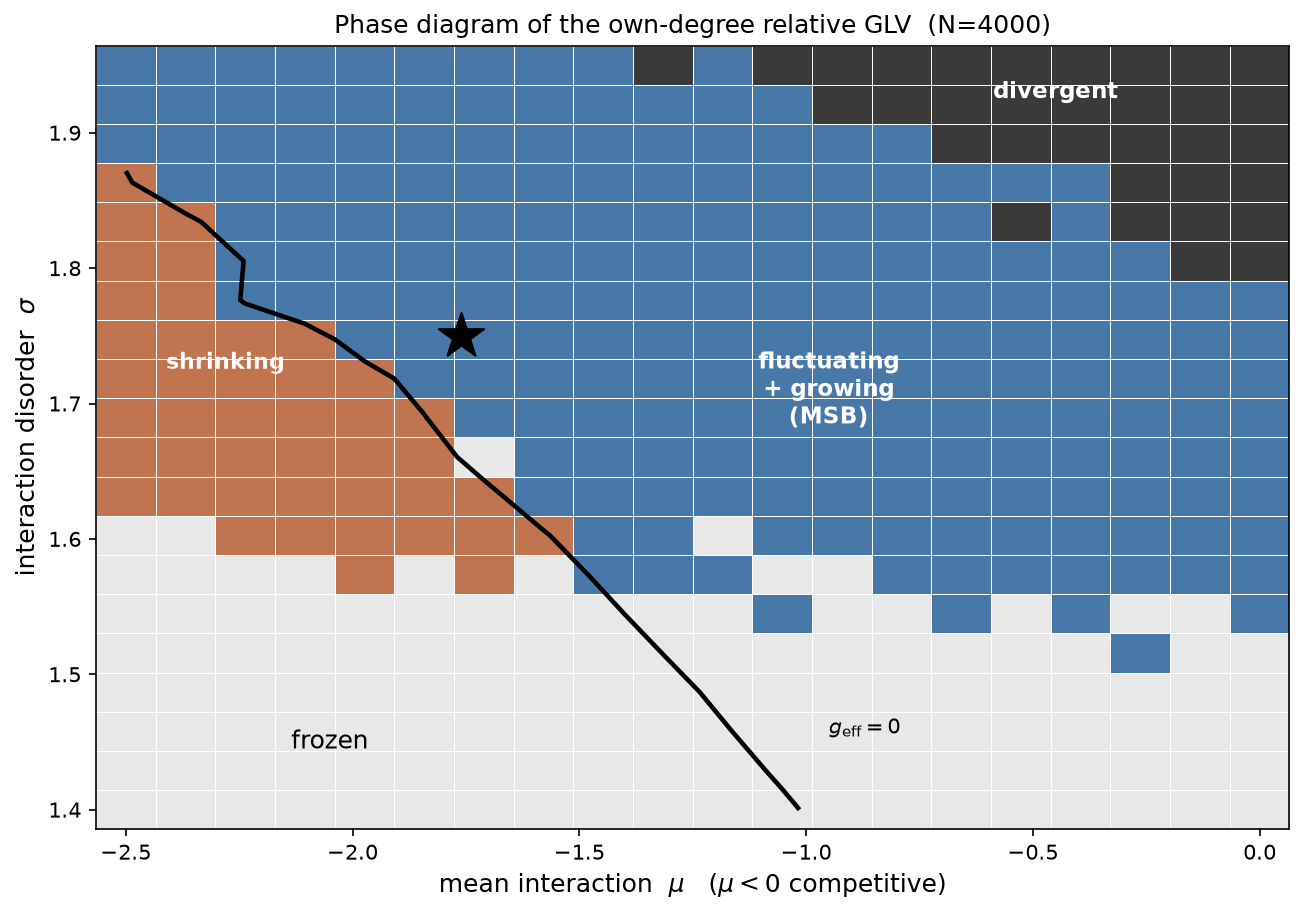
\includegraphics[width=\linewidth]{phase_diagram.png}
    \caption{Phase diagram of the relative model \eqref{eq:relative-glv} under the
    own-degree normalization, over the mean interaction $\mu$ (competitive for $\mu < 0$)
    and the disorder $\sigma$, classified from the late-time dynamics ($N = 4000$, a
    $20 \times 20$ grid with ten realizations per cell). At low disorder the shape relaxes and nothing fluctuates
    (frozen). Above it the dynamics are chaotic, and the solid black line marks the growth
    boundary $g_{\mathrm{eff}} = 0$, which separates the shrinking region ($g_{\mathrm{eff}}
    < 0$) from the fluctuating, growing band in which the firm-growth statistics are
    measured (blue, labelled MSB). The band is bounded below by the freezing line, on the
    competitive side by $g_{\mathrm{eff}} = 0$, and in the strong-disorder corner by the
    explosive, divergent region. The star marks the operating point $\mu = -1.76$,
    $\sigma = 1.75$. The band is an extended region, not a single point.}
    \label{fig:phase-diagram}
\end{figure}

This phase structure is not merely observed but can be derived. The relative model
\eqref{eq:relative-glv} is a disordered replicator equation, and its dynamical mean-field theory,
worked out in Appendix~\ref{app:dmft}, reduces the $N$-firm dynamics to a single representative
firm in a self-consistent Gaussian field. On a regular graph it gives the chaos onset in closed
form, $\sigma_c = \sqrt{2}$, independent of $\mu$. The mean interaction enters every firm's
fitness as the same uniform shift, so it cancels from the replicator and only sets the level of
the growth rate $g_{\mathrm{eff}}$, moving the $g_{\mathrm{eff}} = 0$ line but not the chaos
threshold. Below $\sigma_c$ the relaxed fixed point is the survivor law of the disordered
Lotka--Volterra model with the carrying capacity renormalized by the growth rate, and a direct
simulation on the matching ensemble confirms the predicted growth rate and surviving fraction to
about one percent, the fluctuations switching on exactly at $\sigma_c$. The fluctuating phase
itself, where the firm-growth statistics live, lies beyond this static fixed-point theory and
would need its two-time extension; we measure it directly instead.

Figure~\ref{fig:growing-churn} shows a single run in this regime. The total abundance (left)
climbs as a straight line in $\log M$ over the whole integration, the steady exponential growth
of \eqref{eq:Mdot-relative}, with no sign of a blow-up. The relative firm sizes $S_i = N y_i$
(right) do not settle; after an initial transient they keep exchanging rank and spanning orders
of magnitude, the persistent chaos of the $\sigma > \sigma_c$ phase. The economy grows while its
composition keeps turning over.

\begin{figure}[htbp]
    \centering
    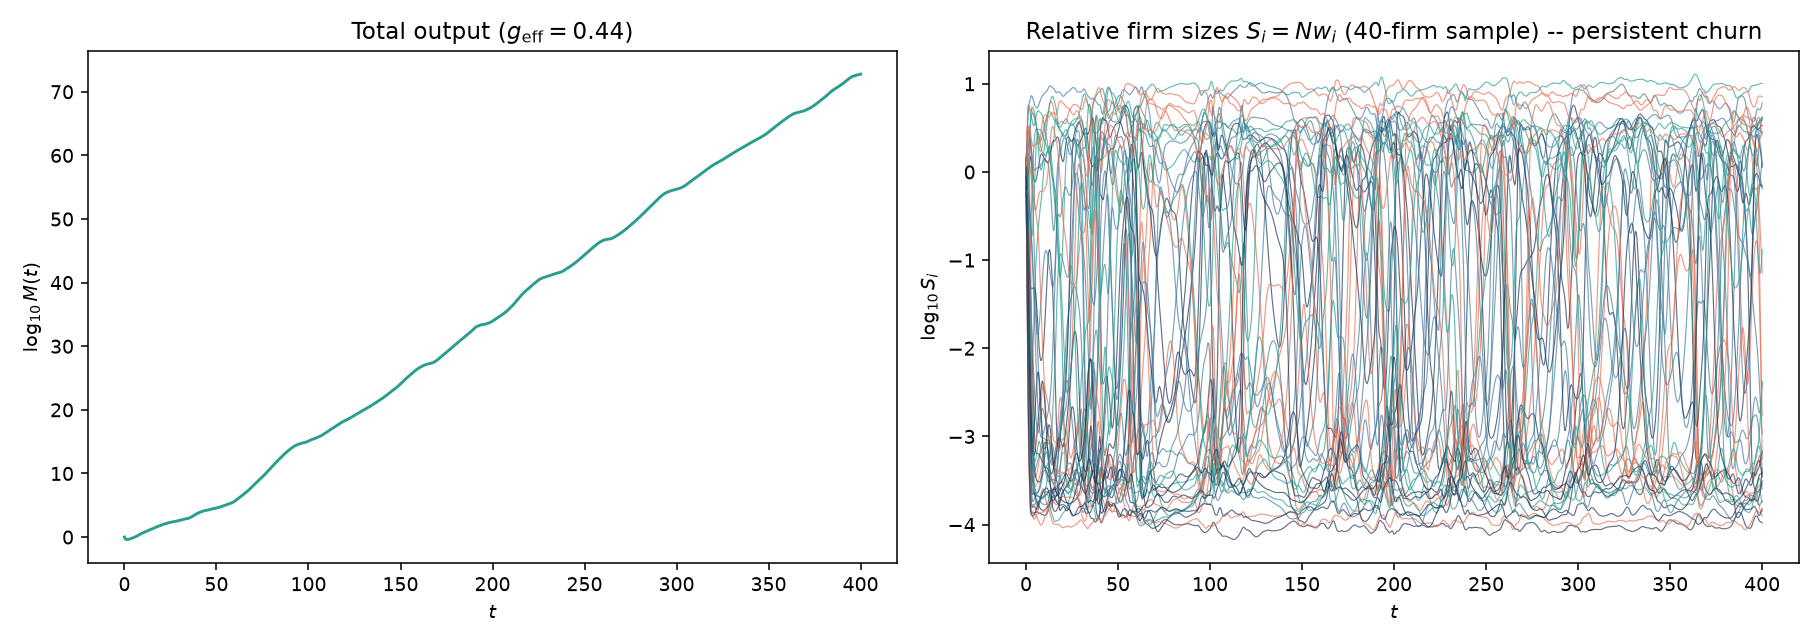
\includegraphics[width=\linewidth]{growing_growth_churn.png}
    \caption{A single run of the relative model \eqref{eq:relative-glv} at $\mu = -1.76$,
    $\sigma = 1.75$, $\lambda = 10^{-3}$ on a power-law graph with $N = 3000$. \panel{Left}: the
    total abundance grows exponentially in physical time, $\log_{10} M(t)$ rising
    linearly, with no finite-time divergence. \panel{Right}: a sample of relative firm sizes
    $S_i = N y_i$, which keep fluctuating and exchanging rank rather than relaxing to a
    fixed point.}
    \label{fig:growing-churn}
\end{figure}
